% ============================================================
%  Mathematischer Artikel – Template
%  Compiler: pdfLaTeX  |  Bibliographie: Biber + BibLaTeX
% ============================================================
\documentclass[12pt, a4paper]{article}

% ── Encoding & Sprache ──────────────────────────────────────
\usepackage[T1]{fontenc}
\usepackage[utf8]{inputenc}
\usepackage[ngerman]{babel}          % ggf. [english] für Englisch

% ── Schrift ─────────────────────────────────────────────────
\usepackage{lmodern}                 % schärfere Schrift als CM

% ── Seitenränder ────────────────────────────────────────────
\usepackage[
  top    = 2.5cm,
  bottom = 2.5cm,
  left   = 2.5cm,
  right  = 2.5cm
]{geometry}

% ── Kopf- und Fußzeile ──────────────────────────────────────
\usepackage{fancyhdr}
\pagestyle{fancy}
\fancyhf{}                           % alle Felder leeren

% Kopfzeile: links Kurztitel, rechts Autor
\fancyhead[L]{\small\itshape Digitale Schachuhr}
\fancyhead[R]{\small Artöm Ederle, Muhammed Esad Özbas, Zeynep Ceren Uncuoglu}

% Fußzeile: mittig Seitenzahl
\fancyfoot[C]{\small\thepage}

% Linie unter Kopfzeile, keine über Fußzeile
\renewcommand{\headrulewidth}{0.4pt}
\renewcommand{\footrulewidth}{0pt}

% ── Mathematik ──────────────────────────────────────────────
\usepackage{amsmath, amssymb, amsthm}
\usepackage{mathtools}               % Erweiterung zu amsmath
\usepackage{thmtools}                % deklarativere Theorem-Umgebungen

% Theorem-Umgebungen
\theoremstyle{plain}
\newtheorem{theorem}{Satz}[section]
\newtheorem{lemma}[theorem]{Lemma}
\newtheorem{proposition}[theorem]{Proposition}
\newtheorem{corollary}[theorem]{Korollar}

\theoremstyle{definition}
\newtheorem{definition}[theorem]{Definition}
\newtheorem{example}[theorem]{Beispiel}

\theoremstyle{remark}
\newtheorem{remark}[theorem]{Bemerkung}

% ── Nützliche Pakete ────────────────────────────────────────
\usepackage[dvipsnames, table]{xcolor} % Farbdefinitionen (vor hyperref laden!)
\usepackage{microtype}               % bessere Typographie
\usepackage{hyperref}                % klickbare Links/Referenzen
\hypersetup{
  colorlinks = true,
  linkcolor  = black,
  citecolor  = blue!60!black,
  urlcolor   = blue!60!black
}
\usepackage{cleveref}                % \cref statt \ref (sprachsensitiv)
\usepackage{enumitem}                % schönere Listen
\usepackage{booktabs}                % schönere Tabellen
\usepackage{graphicx}                % Grafiken einbinden
\usepackage{float}                   % exakte Platzierung von Gleitobjekten

% ── Bibliographie (BibLaTeX + Biber) ────────────────────────
\usepackage[
  backend  = biber,
  style    = alphabetic,             % z. B. [Knu84]; alt: numeric, authoryear
  sorting  = nyt,                    % nach Name, Jahr, Titel
  maxnames = 3
]{biblatex}
\addbibresource{literatur.bib}       % <── Name deiner .bib-Datei

% ── Metadaten ───────────────────────────────────────────────
\title{\textbf{Titel des Artikels}\\[0.5em]
       \large Untertitel (optional)}
\author{Vorname Nachname\\[0.3em]
        \small Institut / Universität\\
        \small \texttt{email@example.com}}
\date{\today}

% ============================================================
\begin{document}

% ── Deckblatt ───────────────────────────────────────────────
\begin{titlepage}
  \centering
  \vspace*{3cm}

  {\LARGE\bfseries Digitale Schachuhr\par}
  \vspace{0.5em}
  {\large Laborbericht Entwurf digitaler Systeme\par}

  \vspace{2.5cm}

  {\large\bfseries Artöm Ederle\\Muhammed Esad Özbas\\Zeynep Ceren Uncuoglu\par}
  \vspace{0.5em}
  {\normalsize DHBW Stuttgart\\[0.3em]\par}

  \vfill

  {\normalsize \today\par}

  \vspace{1.5cm}

  % Abstract auf dem Deckblatt
  \begin{minipage}{0.85\textwidth}
    \small
    \textbf{Abstract.}
    Hier steht eine kurze Zusammenfassung des Artikels (ca.\,5–10 Zeilen).
    Es werden die wichtigsten Resultate genannt und der
    mathematische Kontext skizziert.
  \end{minipage}

  \vspace{1cm}

  % MSC-Klassifikation und Schlüsselwörter (üblich in Math-Artikeln)
  %\begin{minipage}{0.85\textwidth}
  %  \small
  %  \textbf{MSC 2020:} 26A06, 54A05 \quad
  %  \textbf{Schlüsselwörter:} Stichwort eins, Stichwort zwei, Stichwort drei
  %\end{minipage}
\end{titlepage}

% Ab hier greifen Kopf- und Fußzeile
\setcounter{page}{1}

% ============================================================
\section{Einleitung}
Mit dem bereitgestellten Digilent FPGA-Board Basys-3 soll eine digitale Schachuhr realisiert werden. Die vorgegebenen Minimalanforderungen sind:
\begin{itemize}
    \item Zeit von zwei Spielern soll in Minuten und Sekunden angezeigt werden (ohne Richtungsvorgabe)
    \item Spiel soll pausierbar sein
    \item während des laufenden Spiels soll die Zeit umschaltbar sein, wobei die Zeit der entsprechenden Spieler steht bzw. läuft,
    \item es soll ein Reset möglich sein.
\end{itemize}

\section{Realisierung}
Grundsätzlich folgt die Implementierung dem Blockschaltbild in Abbildung \ref{fig:blockschaltbild}.
\begin{figure}[htbp]
  \centering
  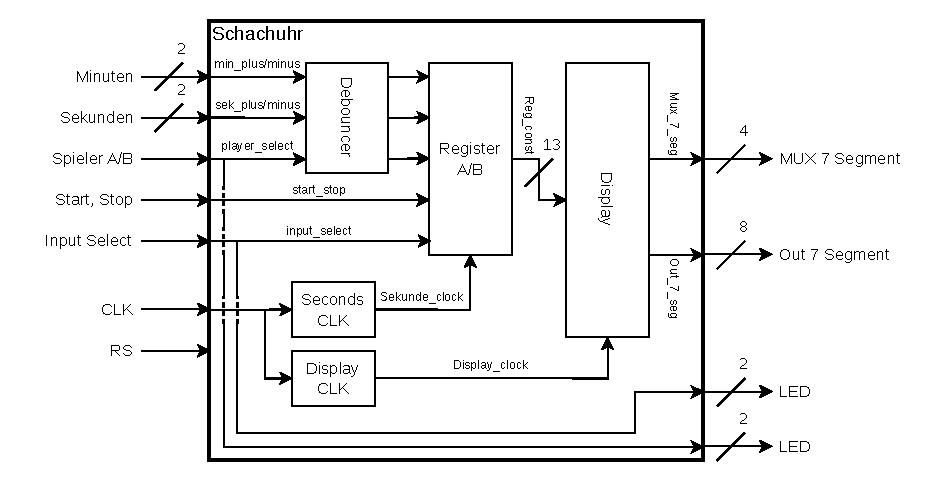
\includegraphics[width=1\textwidth,page=1]{Blockschaltbild.pdf}
  \caption{Blockschaltbild der digitalen Schachuhr.}
  \label{fig:blockschaltbild}
\end{figure}
%
\noindent Die aktuelle Schachuhr umfasst folgende Funktionen, analog zu den offiziellen DGT-2010 Schachuhren:%
\begin{table}[H]
  \centering
  \renewcommand{\arraystretch}{1.2}
\begin{tabular}{|>{\columncolor{gray!15}\bfseries\raggedright\arraybackslash}p{3.6cm}!{\vrule width 1.2pt}p{5.5cm}|p{5.5cm}|}
    \specialrule{1.2pt}{0pt}{0pt}
    \rowcolor{gray!15}
                            & DGT-2010 & Eigene Implementierung\\
    \specialrule{1.2pt}{0pt}{0pt}
    Zeit Einstellbar        & Ja: h, min, s (max.: 99:99:99) & Ja: min, s (max.: 99:99)\\
    \hline
    Inkrement Einstellbar   & Ja: min, s & Ja: min, s \\
    \hline
    Reset & Ein- und Ausschalten der Uhr & in pausiertem Zustand Reset-Taster drücken\\
    \hline
    Verhalten abgelaufene Zeit & Sperrung der Zeit; Markierung mit Flaggensymbol & Sperrung der Zeit; Markierung mit Blinken von Anzeige 00:00\\
    \specialrule{1.2pt}{0pt}{0pt}
  \end{tabular}
  \caption{In der Tabelle sind die Funktionen der eigens implementierten Schachuhr mit denen der offiziellen von der FIDE für Turniere anerkannten Schachuhr DGT-2010.}
  \label{tab:DGT2010vsFPGA}
\end{table}

\noindent Was die Implementierung im Vergleich zur DGT-2010 nicht kann, ist es die gemachten Züge zu zählen. Wenn gewisse Schwellwerte überschritten werden, dann werden zusätzlich eine zweite oder eine dritte Zeit für die Partie zur Verfügung gestellt. 

\section{Ausblick}
Die aktuelle Implementierung kann theoretisch für jegliche Schnellschach- und weitere Zeit-Modi mit kürzerer Dauer verwendet werden. Im Bereich des klassischen Schachs könnte es von den unterschiedlichen etablierten Modi nur den Modus, 90 Minuten für die ganze Partie und 30 Sekunden pro Zug, sprich 30 Sekunden Inkrement.\\

\noindent Im vergangenen Kandidatenturnier 2026 auf Zypern wurde mit dem Modus 120 Minuten für die ersten 40 Züge ohne Inkrement, danach erhalten die Spieler 30 zusätzliche Minuten und ein Inkrement von 30 Sekunden. Dies könnte die aktuelle Implementierung nicht abbilden, aufgrund der fehlenden Zug-Zähler und Zusatzzeiteinstellungen.
\end{document}
%%%%%%%%%%%%%%%%%%%%%%%%%%%%%%%%%%%%%%%%%%%%%%%%%%%%%%%%%%%%%%%%%%%%%%%%%%%%%%%%%%%%%%%%%%%%%%%%%%%%%%%%%%%%%%%%%%%%%%%%%%%%%%%%%%%%%%%%%%%%%%%%%%%%%%%%%%%%%%%%%%%%%%%%%%%%%%%%%%%%%%%%%%%%%%%%%%%%%%%%%%%%%%%%%%%%%%%%%%%%%%%%%%%%%%%%%%%%%%%%%%%%%%%%%%%%%%%%%%%%%%%%%%%%%%%%%%%%%%%%%%%%%%%%%%%%%%
% ============================================================
%  Mathematischer Artikel – Template
%  Compiler: pdfLaTeX  |  Bibliographie: Biber + BibLaTeX
% ============================================================
\documentclass[12pt, a4paper]{article}

% ── Encoding & Sprache ──────────────────────────────────────
\usepackage[T1]{fontenc}
\usepackage[utf8]{inputenc}
\usepackage[ngerman]{babel}          % ggf. [english] für Englisch

% ── Schrift ─────────────────────────────────────────────────
\usepackage{lmodern}                 % schärfere Schrift als CM

% ── Seitenränder ────────────────────────────────────────────
\usepackage[
  top    = 2.5cm,
  bottom = 2.5cm,
  left   = 2.5cm,
  right  = 2.5cm
]{geometry}

% ── Kopf- und Fußzeile ──────────────────────────────────────
\usepackage{fancyhdr}
\pagestyle{fancy}
\fancyhf{}                           % alle Felder leeren

% Kopfzeile: links Kurztitel, rechts Autor
\fancyhead[L]{\small\itshape Digitale Schachuhr}
\fancyhead[R]{\small Artöm Ederle, Muhammed Esad Özbas, Zeynep Ceren Uncuoglu}

% Fußzeile: mittig Seitenzahl
\fancyfoot[C]{\small\thepage}

% Linie unter Kopfzeile, keine über Fußzeile
\renewcommand{\headrulewidth}{0.4pt}
\renewcommand{\footrulewidth}{0pt}

% ── Mathematik ──────────────────────────────────────────────
\usepackage{amsmath, amssymb, amsthm}
\usepackage{mathtools}               % Erweiterung zu amsmath
\usepackage{thmtools}                % deklarativere Theorem-Umgebungen

% Theorem-Umgebungen
\theoremstyle{plain}
\newtheorem{theorem}{Satz}[section]
\newtheorem{lemma}[theorem]{Lemma}
\newtheorem{proposition}[theorem]{Proposition}
\newtheorem{corollary}[theorem]{Korollar}

\theoremstyle{definition}
\newtheorem{definition}[theorem]{Definition}
\newtheorem{example}[theorem]{Beispiel}

\theoremstyle{remark}
\newtheorem{remark}[theorem]{Bemerkung}

% ── Nützliche Pakete ────────────────────────────────────────
\usepackage[dvipsnames, table]{xcolor} % Farbdefinitionen (vor hyperref laden!)
\usepackage{microtype}               % bessere Typographie
\usepackage{hyperref}                % klickbare Links/Referenzen
\hypersetup{
  colorlinks = true,
  linkcolor  = black,
  citecolor  = blue!60!black,
  urlcolor   = blue!60!black
}
\usepackage{cleveref}                % \cref statt \ref (sprachsensitiv)
\usepackage{enumitem}                % schönere Listen
\usepackage{booktabs}                % schönere Tabellen
\usepackage{graphicx}                % Grafiken einbinden
\usepackage{float}                   % exakte Platzierung von Gleitobjekten

% ── Bibliographie (BibLaTeX + Biber) ────────────────────────
\usepackage[
  backend  = biber,
  style    = alphabetic,             % z. B. [Knu84]; alt: numeric, authoryear
  sorting  = nyt,                    % nach Name, Jahr, Titel
  maxnames = 3
]{biblatex}
\addbibresource{literatur.bib}       % <── Name deiner .bib-Datei

% ── Metadaten ───────────────────────────────────────────────
\title{\textbf{Titel des Artikels}\\[0.5em]
       \large Untertitel (optional)}
\author{Vorname Nachname\\[0.3em]
        \small Institut / Universität\\
        \small \texttt{email@example.com}}
\date{\today}

% ============================================================
\begin{document}

% ── Deckblatt ───────────────────────────────────────────────
\begin{titlepage}
  \centering
  \vspace*{3cm}

  {\LARGE\bfseries Digitale Schachuhr\par}
  \vspace{0.5em}
  {\large Laborbericht Entwurf digitaler Systeme\par}

  \vspace{2.5cm}

  {\large\bfseries Artöm Ederle\\Muhammed Esad Özbas\\Zeynep Ceren Uncuoglu\par}
  \vspace{0.5em}
  {\normalsize DHBW Stuttgart\\[0.3em]\par}

  \vfill

  {\normalsize \today\par}

  \vspace{1.5cm}

  % Abstract auf dem Deckblatt
  %\begin{minipage}{0.85\textwidth}
  %  \small
  %  \textbf{Abstract.}
  %  Hier steht eine kurze Zusammenfassung des Artikels (ca.\,5–10 Zeilen).
  %  Es werden die wichtigsten Resultate genannt und der
  %  mathematische Kontext skizziert.
  %\end{minipage}

  \vspace{1cm}

  % MSC-Klassifikation und Schlüsselwörter (üblich in Math-Artikeln)
  %\begin{minipage}{0.85\textwidth}
  %  \small
  %  \textbf{MSC 2020:} 26A06, 54A05 \quad
  %  \textbf{Schlüsselwörter:} Stichwort eins, Stichwort zwei, Stichwort drei
  %\end{minipage}
\end{titlepage}

% Ab hier greifen Kopf- und Fußzeile
\setcounter{page}{1}

% ============================================================
\section{Einleitung}
Mit dem bereitgestellten Digilent FPGA-Board Basys-3 soll eine digitale Schachuhr realisiert werden. Die vorgegebenen Minimalanforderungen sind:
\begin{itemize}
    \item Zeit von zwei Spielern soll in Minuten und Sekunden angezeigt werden (ohne Richtungsvorgabe)
    \item Spiel soll pausierbar sein
    \item während des laufenden Spiels soll die Zeit umschaltbar sein, wobei die Zeit der entsprechenden Spieler steht bzw. läuft,
    \item es soll ein Reset möglich sein.
\end{itemize}

\section{Realisierung}
Grundsätzlich folgt die Implementierung dem Blockschaltbild in Abbildung \ref{fig:blockschaltbild}.
\begin{figure}[htbp]
  \centering
  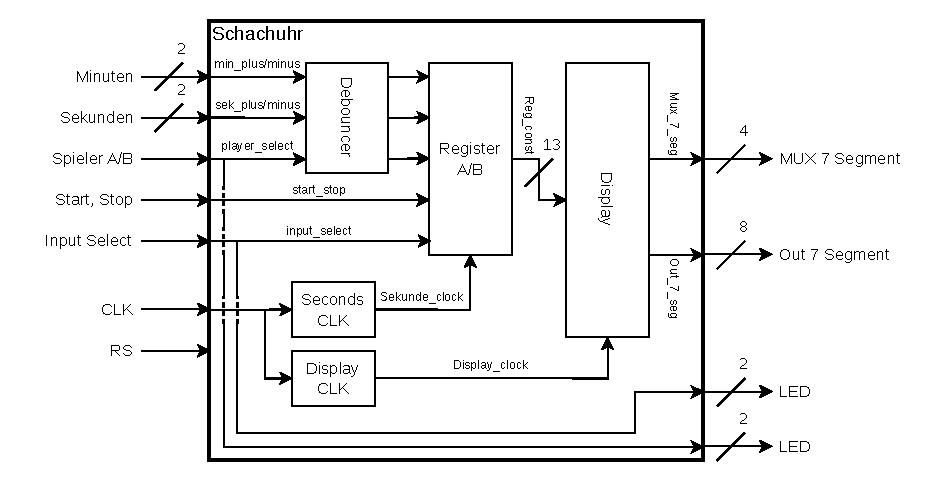
\includegraphics[width=1\textwidth,page=1]{Blockschaltbild.pdf}
  \caption{Blockschaltbild der digitalen Schachuhr.}
  \label{fig:blockschaltbild}
\end{figure}
%
\noindent Die aktuelle Schachuhr umfasst folgende Funktionen, analog zu den offiziellen DGT-2010 Schachuhren:%
\begin{table}[H]
  \caption{In der Tabelle werden die Funktionen der eigens implementierten Schachuhr denen der offiziell von der FIDE anerkannten Schachuhr DGT-2010 gegenübergestellt.}
  \centering
  \renewcommand{\arraystretch}{1.2}
\begin{tabular}{|>{\columncolor{gray!15}\bfseries\raggedright\arraybackslash}p{3.6cm}!{\vrule width 1.2pt}p{5.5cm}|p{5.5cm}|}
    \specialrule{1.2pt}{0pt}{0pt}
    \rowcolor{gray!15}
                            & DGT-2010 & Eigene Implementierung\\
    \specialrule{1.2pt}{0pt}{0pt}
    Zeit Einstellbar        & Ja: h, min, s (max.: 99:99:99) & Ja: min, s (max.: 99:99)\\
    \hline
    Inkrement Einstellbar   & Ja: min, s & Ja: min, s \\
    \hline
    Reset & Ein- und Ausschalten der Uhr & in pausiertem Zustand Reset-Taster drücken\\
    \hline
    Verhalten abgelaufene Zeit & Sperrung der Zeit; Markierung mit Flaggensymbol & Sperrung der Zeit; Markierung mit Blinken von Anzeige 00:00\\
    \specialrule{1.2pt}{0pt}{0pt}
  \end{tabular}
  
  \label{tab:DGT2010vsFPGA}
\end{table}

%\noindent Was die Implementierung im Vergleich zur DGT-2010 nicht kann, ist es die gemachten Züge zu zählen und entsprechende Zusatzzeiten einzustellen. Wenn gewisse Schwellwerte, z.B. nach 40 Zügen, überschritten werden, dann werden zusätzlich z.B. 30 Minuten für die Partie zur Verfügung gestellt. 

\section{Ausblick}
Die aktuelle Implementierung kann theoretisch für jegliche Schnellschach- und weitere Zeit-Modi mit kürzerer Dauer verwendet werden. Im Bereich des klassischen Schachs könnte es von den unterschiedlichen etablierten Modi nur den Modus, 90 Minuten für die ganze Partie und 30 Sekunden pro Zug, sprich 30 Sekunden Inkrement, realisieren.\\

\noindent Im vergangenen Kandidatenturnier 2026 auf Zypern wurde mit dem Modus 120 Minuten für die ersten 40 Züge ohne Inkrement, danach erhalten die Spieler 30 zusätzliche Minuten und ein Inkrement von 30 Sekunden. Dies könnte die aktuelle Implementierung nicht abbilden, aufgrund der fehlenden Zug-Zähler und Zusatzzeiteinstellungen.
\end{document}
